%
\section{Introduction}%
%
\begin{frame}[t]%
\frametitle{Introduction}%
\bigskip%
\begin{itemize}%
\item Benchmarking of optimization algorithms is \only<2->{incredibly }important\uncover<3->{, but cumbersome}%
\item<4-> Tool support is needed\uncover<5->{, examples are \bbob's \coco\expandafter\scitep{\cocoReferences}, \tspSuite\scitep{\tspSuiteReferences}, \frameworkStyle{UBCSAT}\scitep{TH2004UAIAEEFSAFSAMS}, or \frameworkStyle{AOAB}\scitep{WNT2010AOABAOAB}\uncover<6->{ -- \textcolor<6>{red}{which are all \inQuotes{field-specific}}}}
\item<7-> Can we design a general tool for evaluating results from experiments with optimization algorithms?%
\\~\bigskip~\\\bigskip~\\\bigskip~\\\medskip%
\item<8-> {\textbf{\Large{\alert{\optimizationBenchmarking\ is an attempt to do just that.}}}}%
\end{itemize}%
\locateFramedGraphic{8}{width=0.4\paperwidth}{graphics/logo/logo}{0.3}{0.2}%
\end{frame}%
%
\begin{frame}[t]%
\frametitle{Experimental Procedure}%
\begin{itemize}%
\item In optimization or Machine Learning, the following experimental procedure is often used\uncover<2->{%
\begin{enumerate}%
\item Select a set of benchmark instances which covers some \textcolor<20>{red}{different problem features}\only<3>{:%
\begin{itemize}%
\item e.g., \bbob\expandafter\scitep{\bbobReferences} offers different benchmark functions for numerical optimization problems%
\end{itemize}%
}%
\item<5-> Do experiments\only<11->{ with \textcolor<20>{red}{different algorithms/setups}}\only<6-10>{:%
\begin{itemize}%
\item several independent runs of algorithm for each benchmark instance%
\item<7-> collect algorithm progress information, e.g., as \emph{\inQuotes{runtime - bestObjectiveValue}} tuples%
\item<8-> one log file per run, each log file has several such tuples%
\item<9-> repeat for different algorithm parameter settings (e.g., different population sizes of an EA)%
\item<10-> repeat with other algorithms for comparison purposes%
\end{itemize}%
}%
\item<12-> Evaluate the gathered data\only<13->{:%
\begin{itemize}%
\item \textcolor<19>{green}{draw diagrams of progress of solution quality over time}%
\item<14-> \textcolor<19>{green}{draw diagrams of advanced statistical parameters such as ECDF\scitep{HAFR2012RPBBOBES,HS1998ELVAPAR,TH2004UAIAEEFSAFSAMS,WCTLTCMY2014BOAAOSFFTTSP}\only<15->{ and ERT\scitep{HAFR2012RPBBOBES,WCTLTCMY2014BOAAOSFFTTSP}} (over time)}%
\item<16-> use statistical tests to compare results (at different points during the runs)\only<19>{ \textcolor<19>{green}{(soon to come)}}%
\item<17-> analyze the impact of benchmark features and algorithm parameters on the above\only<19>{ \textcolor<19>{green}{(soon to come)}}%
\end{itemize}%
}%
%
\item<18-> But this is all \emph{very} cumbersome, involves much work and much data\dots%
\end{enumerate}%
}%
\item<19-> \alert{The \optimizationBenchmarking\ framework \textcolor<19>{green}{can automatize} much of the evaluation procedure}%
\item<20-> {\dots}and make use of \textcolor<20>{red}{meta-data} about experiments to group and aggregate information.% 
\end{itemize}%
%
\locateWithCaption{3}{%
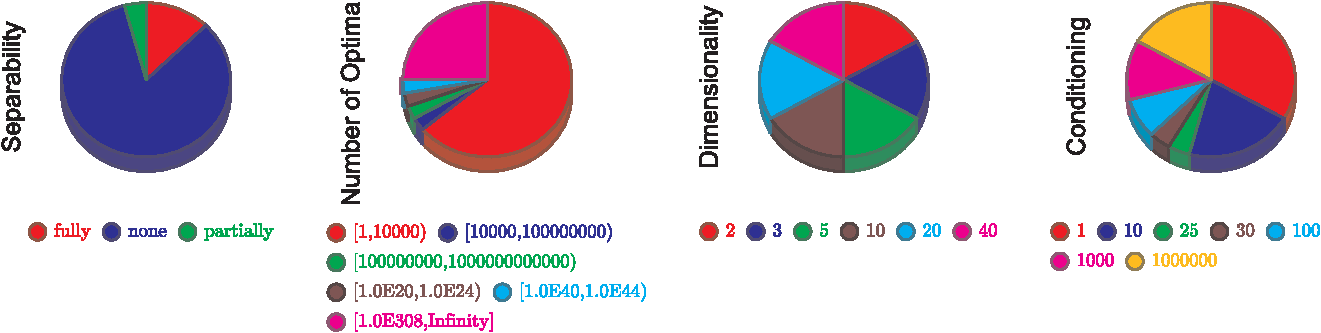
\includegraphics[width=0.925\paperwidth]{graphics/bbob_features/bbob_features}%
}{%
The relative amounts of \bbob\expandafter\scitep{\bbobReferences} benchmark functions according to their features.%
}{0.0375}{0.51}{0.925}%
%
\locateWithCaption{7-8}{%
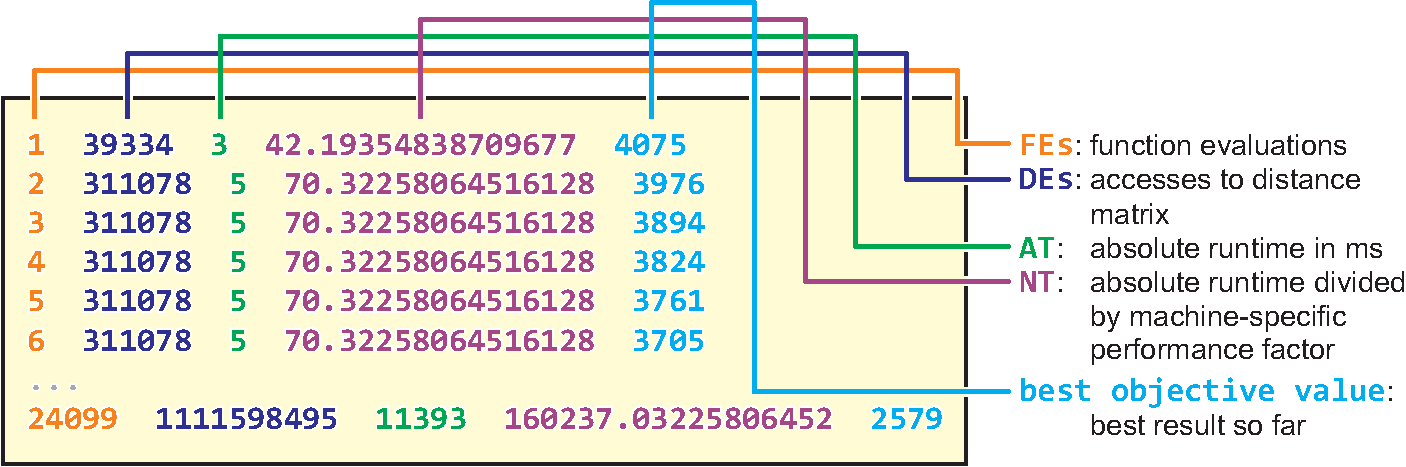
\includegraphics[width=0.8\paperwidth]{graphics/tspSuite_logfile_example/tspSuite_logfile_example}%
}{%
Example for data collected in a log file by \tspSuite\expandafter\scitep{\tspSuiteReferences}.%
}{0.0375}{0.53}{0.925}%
%
\locateWithCaption{13-15}{
\strut%
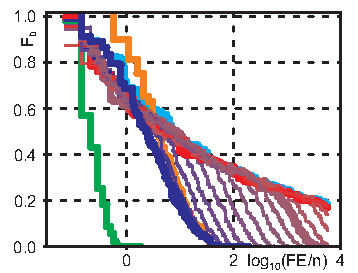
\includegraphics[width=0.28\paperwidth]{graphics/performance/progress_example/progress_example}%
\uncover<14->{%
\strut\hfill\strut%
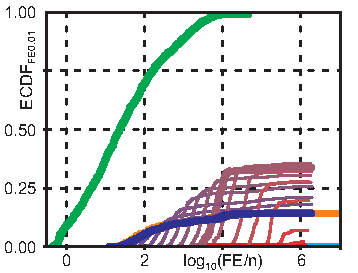
\includegraphics[width=0.28\paperwidth]{graphics/performance/ecdf_example/ecdf_example}%
\uncover<15->{%
\strut\hfill\strut%
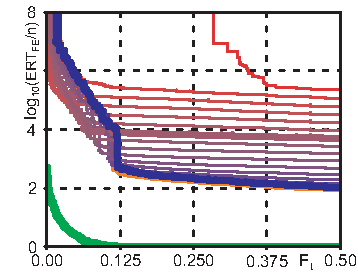
\includegraphics[width=0.28\paperwidth]{graphics/performance/ert_example/ert_example}%
}}\strut%
}{%
Examples for progress\only<14->{ and ERT}\only<15->{, ERT, and ECDF} diagrams from \tspSuite\expandafter\scitep{\tspSuiteReferences} for different algorithms (signified by different colors) over different sub-sets of the \tspLib\expandafter\scitep{\tspLibReferences} data.%
}{0.0375}{0.545}{0.925}%
%
\end{frame}%
